\documentclass[../report/main.tex]{subfiles}
 
\begin{document}

\begin{enumerate}[a)]
	\item What are the lengths of the shortest paths from vertex $a$ to all other vertices?

    The shortest path problem can be solved using the following linear programming formulation:

  \begin{equation*}
    \begin{aligned}
      % Minimize path length
      & \text{minimize} & & -d_t \\
      & \text{subject to} & & d_s = 0 \\
      & & & d_v - d_u \leq \ell(uv) \quad \forall \text{ edges } uv \\
      & & & -d_u \leq 0 \quad \forall \text{ vertices } u \in V
    \end{aligned}
  \end{equation*}

  Based on the vertices and weights provided in the Project3Problem3-1.txt file, the constraints for the linear programming formulation to find shortest paths will be:

  \begin{itemize}
    \item $d_b - d_a \leq 2$
    \item $d_c - d_a \leq 3$
    \item $d_d - d_a \leq 8$
    \item $d_h - d_a \leq 9$
    \item $d_a - d_b \leq 4$
    \item $d_c - d_b \leq 5$
    \item $d_e - d_b \leq 7$
    \item $d_f - d_b \leq 4$
    \item $d_d - d_c \leq 10$
    \item $d_b - d_c \leq 5$
    \item $d_g - d_c \leq 9$
    \item $d_i - d_c \leq 11$
    \item $d_f - d_c \leq 4$
    \item $d_a - d_d \leq 8$
    \item $d_g - d_d \leq 2$
    \item $d_j - d_d \leq 5$
    \item $d_f - d_d \leq 1$
    \item $d_h - d_e \leq 5$
    \item $d_c - d_e \leq 4$
    \item $d_i - d_e \leq 10$
    \item $d_i - d_f \leq 2$
    \item $d_g - d_f \leq 2$
    \item $d_d - d_g \leq 2$
    \item $d_j - d_g \leq 8$
    \item $d_k - d_g \leq 12$
    \item $d_i - d_h \leq 5$
    \item $d_k - d_h \leq 10$
    \item $d_a - d_i \leq 20$
    \item $d_k - d_i \leq 6$
    \item $d_j - d_i \leq 2$
    \item $d_m - d_i \leq 12$
    \item $d_i - d_j \leq 2$
    \item $d_k - d_j \leq 4$
    \item $d_l - d_j \leq 5$
    \item $d_h - d_k \leq 10$
    \item $d_m - d_k \leq 10$
    \item $d_m - d_l \leq 2$
  \end{itemize}

  An image of the digraph is below:

  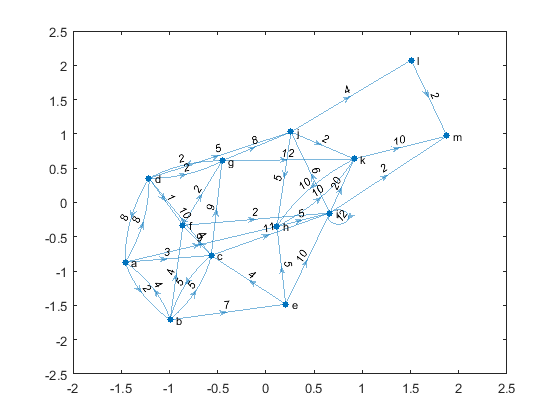
\includegraphics{../problem_three/img/problem3_digraph.png}

  The MATLAB function \verb|linprog| was utilized to find the solution. The following are the lengths of the shortest paths from $a$ to each of the other vertices in the graph. \\
  
  \lstinputlisting{../problem_three/matlab/P3A_solution.txt}

  The following MATLAB code was used to generate the solution.

  \lstinputlisting{../problem_three/matlab/problem3_partA.m}

  \newpage

	\item If a vertex $z$ is added to the graph for which there is no path from vertex $a$ to vertex $z$, what will be the result when you attempt to find the lengths of shortest paths as in part a).

  Consider the following possible digraph with unreachable $z$:

  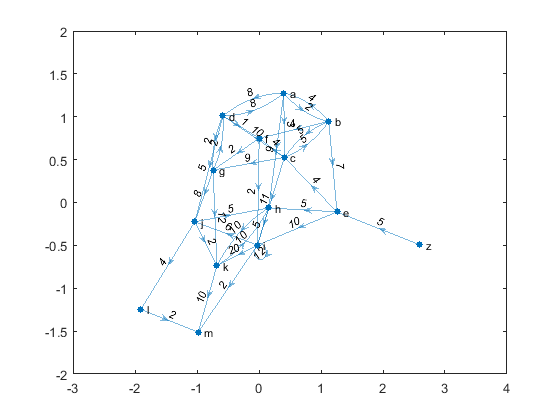
\includegraphics{../problem_three/img/problem3_digraph_with_z.png}

  %\lstinputlisting{../problem_three/matlab/problem3_partB.m}

  The solution code is the same as was presented in part (a). When the code is run, the following error message is presented: \\

  \begin{verbatim}
  Exiting: One or more of the residuals, duality gap, or total relative error
  has stalled:
         the dual appears to be infeasible and the primal unbounded since
         the primal objective < -1e+10
         and the dual objective < 1e+6.
  \end{verbatim}

  The error message is saying that the optimization function has failed to converge on a solution because the new vertex $z$ is unreachable. It is not feasible to find the shortest path to an unreachable vertex.

  There are two possible work-arounds for this problem. The first step in either method is to identify the vertex that the optimization routine is having difficulties with. You can determine this by examining the preliminary values for the distance to each vertex. The unreachable vertices will have very large values.

  The first approach is to remove the unreachable vertices from your optimization function. Suppose you had vertices $a$, $b$, $c$, and $d$, with vertex $d$ being unreachable from $a$. You could simply change your optimization statement from:

  \begin{equation*}
    \begin{aligned}
      % Minimize calories
      & \text{minimize} & & -d_a - d_b - d_c - d_d \\
    \end{aligned}
  \end{equation*}

  to the form:

  \begin{equation*}
    \begin{aligned}
      % Minimize calories
      & \text{minimize} & & -d_a - d_b - d_c \\
    \end{aligned}
  \end{equation*}

  This allows the optimization routine to find a feasible solution.

  Another alernative approach is to specify the distance of the unreachable vertices to be a very large value (large being relative to the maximum path length in the graph) using an equality constraint. By fixing the value, you essentially remove it from consideration by the optimization routine. By giving it a large value, you ensure that it will not conflict in any way with the optimal result. In post processing of the results, you would note that the fixed value you provided denoted that the vertex was unreachable.

  Following either of these methods would then yield the same result as in part (a).

  \newpage

	\item What are the lengths of the shortest paths from each vertex to vertex $m$? How can you solve this problem with just one linear program?

  Finding the shortest path from each vertex to the vertex $m$ is equivalent to flipping the directionality of each edge, and then finding the shortest path from $m$ to each vertex. The resulting path lengths are equivalent to the distance from a given vertex to $m$ with the original edge directions.

  The MATLAB function \verb|linprog| was utilized to find the solution. The following are the lengths of the shortest paths from each vertex to $m$.\\
    
  \lstinputlisting{../problem_three/matlab/P3C_solution.txt}

  The following MATLAB code was used to generate the solution.

  \lstinputlisting{../problem_three/matlab/problem3_partC.m}
    
  \newpage

	\item Suppose that all paths must pass through vertex $i$. How can you calculate the length of the shortest path from any vertex $x$ to vertex $y$ that pass through vertex $i$ (for all $x, y \in V$)? Calculate the lengths of these paths for the given graph. (Note: for some vertices $x$ and $y$, it may be impossible to pass through vertex $i$).

  The length of the shortest path from any vertex $x$ to any vertex $y$ that passes through the vertex $i$ is equivalent to:

  \[
    (\text{Shortest path from } x \text{ to } i) + (\text{Shortest path from } i \text{ to } y)
  \]

  The first term in this equation is equivalent to part (c) of this problem - find the shortest path from each vertex to a given vertex. The second term in this equation is equivalent to part (a) of this problem - find the shortest path from a given vertex to each other vertex.

  In the first portion, there are two vertices that are unable to reach vertex $i$. Looking back at the graphical representation of the digraph in part (a), it's easy to see that these vertices are $l$ and $m$. $l$ is only able to reach vertex $m$, and vertex $m$ is unable to reach any other vertex. In the second portion, all vertices are accessible from vertex $i$.

  The MATLAB function \verb|linprog| was utilized to find the solution for each aspect of the problem (distances to i, and distances from i). The following are the lengths of the shortest paths from each vertex to every other vertex, passing through vertex $i$. A distance of \verb|NaN| denotes that there is not a path between the vertices that travels through vertex $i$. \\

  \lstinputlisting{../problem_three/matlab/P3D_solution.txt}

  The following MATLAB code was used to generate the solution.

  \lstinputlisting{../problem_three/matlab/problem3_partD.m}

    
\end{enumerate}

\end{document}
